\begin{table*}[p]

\begin{multicols}{2}
\noindent
{\scriptsize\begin{sftabular}{@{}m{.05\columnwidth} m{.1\textwidth} m{.63\columnwidth}@{}}
\toprule
\multicolumn{2}{@{}l@{}}{\textbf{Schlüssel}} &  \textbf{Kurzbeschreibung} \\
\midrule
01.1 & 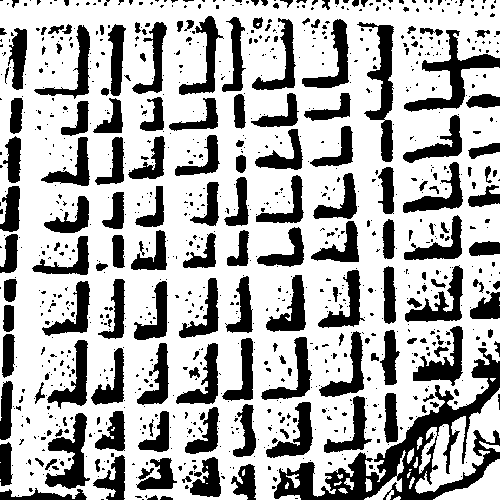
\includegraphics[width=.1\textwidth]{tbl/Tab_VerzElemente/V03a_PIK87-1-7-1.png} & \textit{Schachbrett}-Muster aus horizontalen und vertikalen Ritzlinien \\
01.2 & 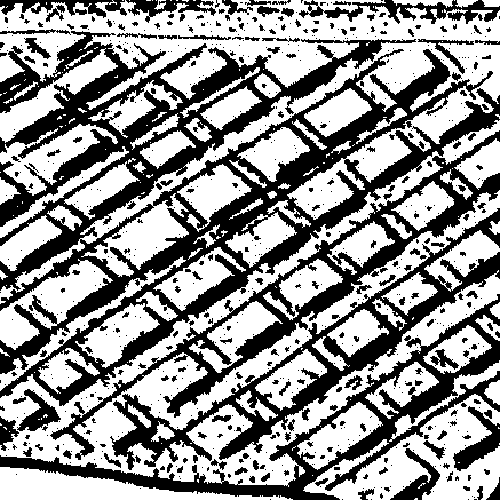
\includegraphics[width=.1\textwidth]{tbl/Tab_VerzElemente/V03b_PIK87-1-6-16.png} & \textit{Schachbrett}-Muster aus diagonalen Ritzlinien \\
01.3 & 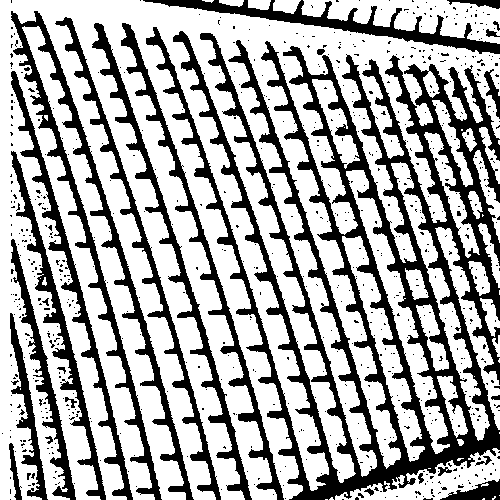
\includegraphics[width=.1\textwidth]{tbl/Tab_VerzElemente/V03c_PIK87-1-8-6.png} & \textit{Schachbrett}-Muster aus horizontalen und diagonalen Ritzlinien \\
01.4 & 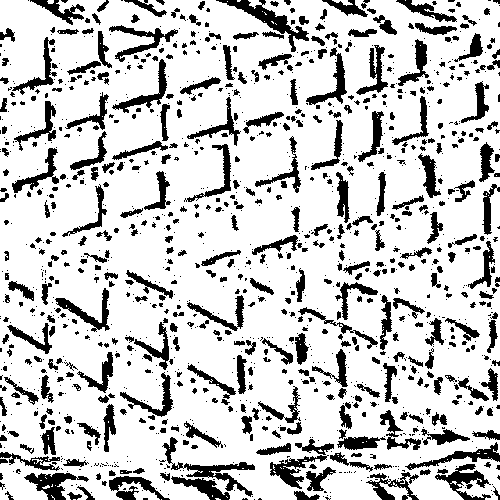
\includegraphics[width=.1\textwidth]{tbl/Tab_VerzElemente/V03d_PIK87-1-9-7.png} & \textit{Schachbrett}-Muster aus diagonalen und vertikalen Ritzlinien \\
01.5 & 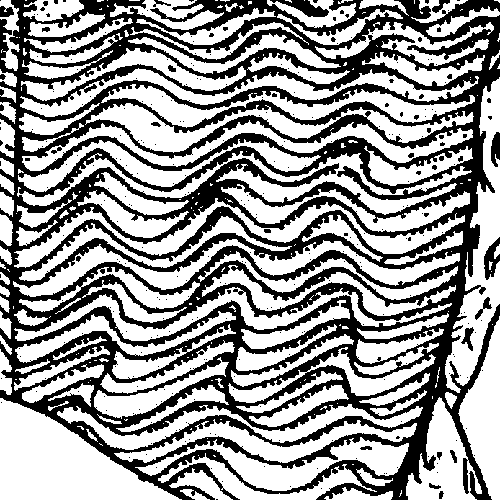
\includegraphics[width=.1\textwidth]{tbl/Tab_VerzElemente/V01b_PIK87-1-5-7.png} & Wellenlinien \\
01.6 & 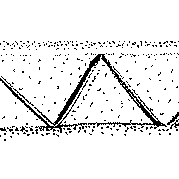
\includegraphics[width=.1\textwidth]{tbl/Tab_VerzElemente/V12a1_MSG87-102-8.png} & Zickzack-Linien \\
01.7 & 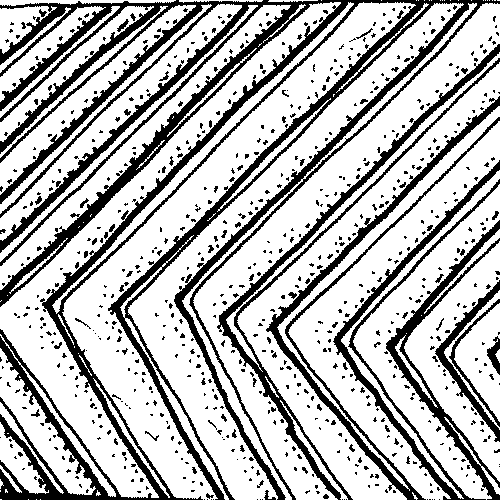
\includegraphics[width=.1\textwidth]{tbl/Tab_VerzElemente/V12c_Gef9_CAM07-3-1-278-306.png} & Rillen in Fischgrät-Muster \\
01.8 & 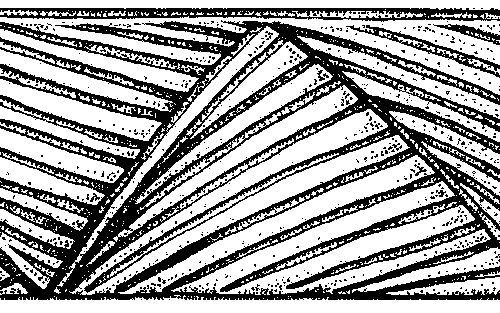
\includegraphics[width=.1\textwidth]{tbl/Tab_VerzElemente/V04d_PIK87-101-43-46.png} 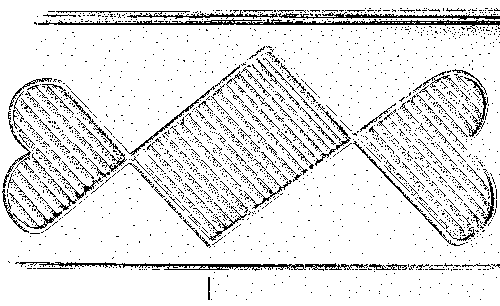
\includegraphics[width=.1\textwidth]{tbl/Tab_VerzElemente/V04e_NGO87-102-28-29.png} & Rillen gefüllte Flächen (Dreiecke, Rauten u.~a.) \\
01.9 & 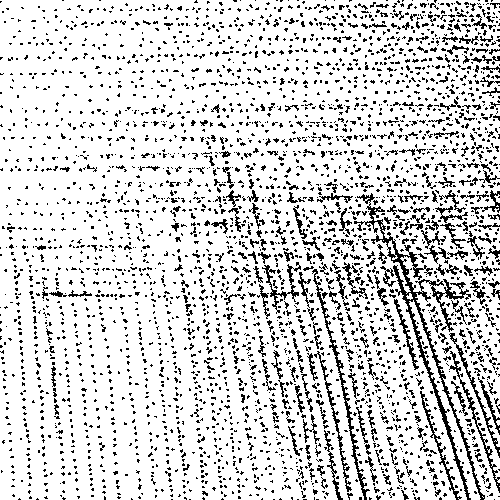
\includegraphics[width=.1\textwidth]{tbl/Tab_VerzElemente/V10a_PIK87-101-51.png} & feine vertikale oder horizontale Rillen \\
01.10 & 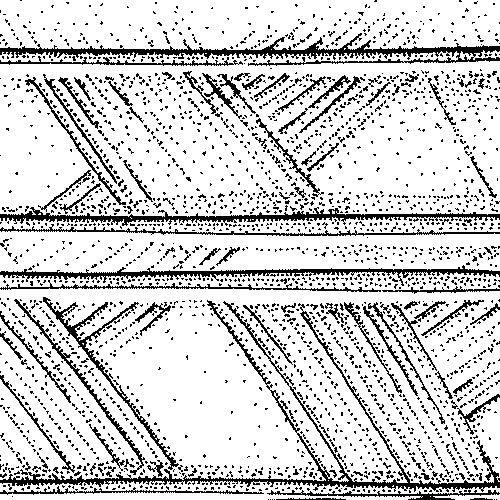
\includegraphics[width=.1\textwidth]{tbl/Tab_VerzElemente/V10b_PIK87-101-40.png} & feine diagonale Rillen \\
01.11 & 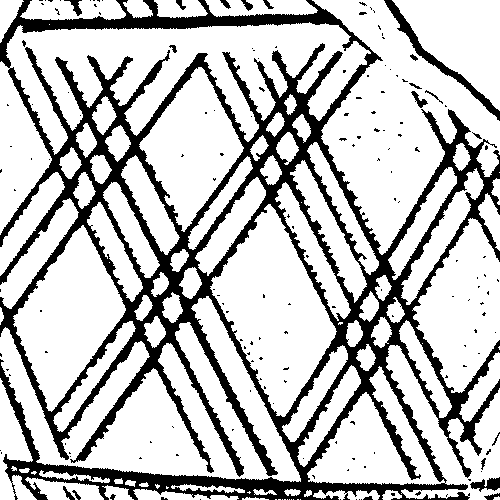
\includegraphics[width=.1\textwidth]{tbl/Tab_VerzElemente/V11b1_LKW87-186-1-2-5.png} & Muster aus überkreuzten Rillen \\
02.1 & 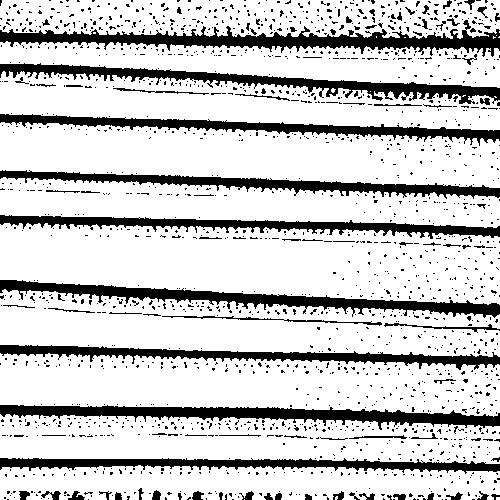
\includegraphics[width=.1\textwidth]{tbl/Tab_VerzElemente/V01a_PIK87-1-8-6.png} & horizontale Riefen \parencite[siehe Muster \enquote{ISpeg5} von][251 Abb. 30.5 ]{GouemGouem.20102011} \\
02.2 & 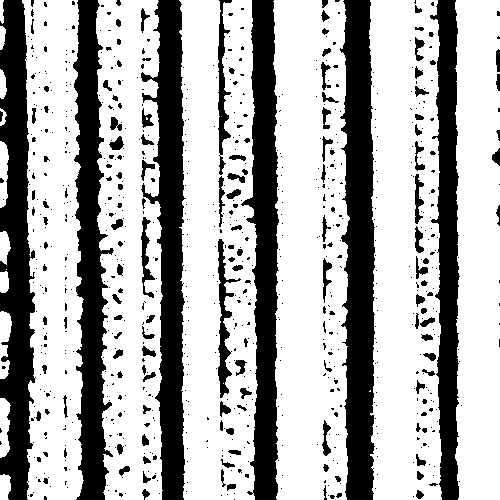
\includegraphics[width=.1\textwidth]{tbl/Tab_VerzElemente/V01c_PIK87-1-8-6.png} & vertikale Riefen \\
\bottomrule
\end{sftabular}}

\noindent
{\scriptsize\begin{sftabular}{@{}m{.05\columnwidth} m{.1\textwidth} m{.63\columnwidth}@{}}
\toprule
\multicolumn{2}{@{}l@{}}{\textbf{Schlüssel}} &  \textbf{Kurzbeschreibung} \\
\midrule
02.3 & 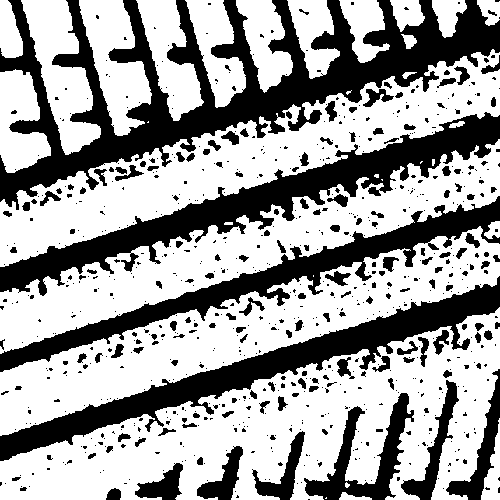
\includegraphics[width=.1\textwidth]{tbl/Tab_VerzElemente/V01e_PIK87-1-8-6.png} & diagonale Riefen \\
02.4 & 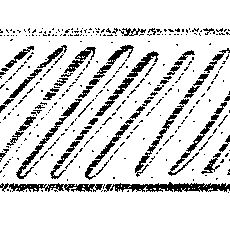
\includegraphics[width=.1\textwidth]{tbl/Tab_VerzElemente/V01e2_MLB85-1-3-2-5-35.png} & horizontales Band aus kurzen diagonalen Riefen \\
02.5 & 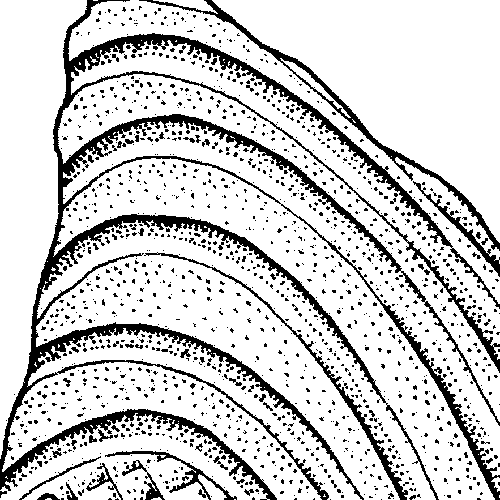
\includegraphics[width=.1\textwidth]{tbl/Tab_VerzElemente/V01d_PIK87-101-7.png} & gebogene Riefen \\
02.6 & 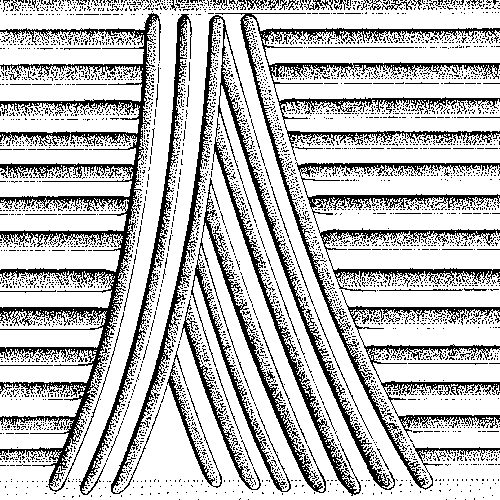
\includegraphics[width=.1\textwidth]{tbl/Tab_VerzElemente/V01f_MUN87-2-1-1-5-2.png} & spitz zusammenlaufende gebogene Riefen \\
02.7 & 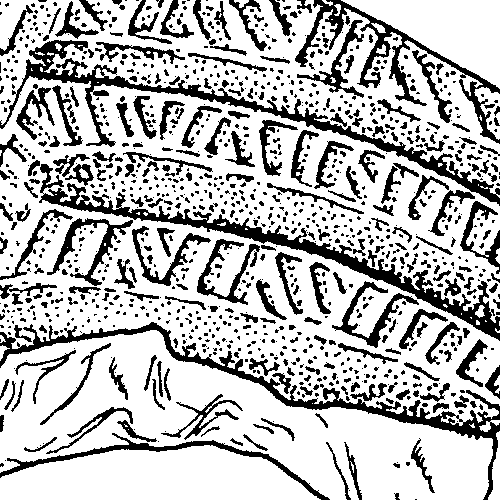
\includegraphics[width=.1\textwidth]{tbl/Tab_VerzElemente/V04c_PIK87-1-3-9.png} & sehr breite Riefen (\textgreater\,5\,mm) \\
03.1 & 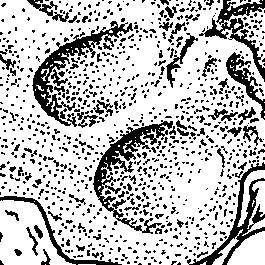
\includegraphics[width=.1\textwidth]{tbl/Tab_VerzElemente/V06e.png} & große Eindrücke, Fingereindrücke \\
04.1 & 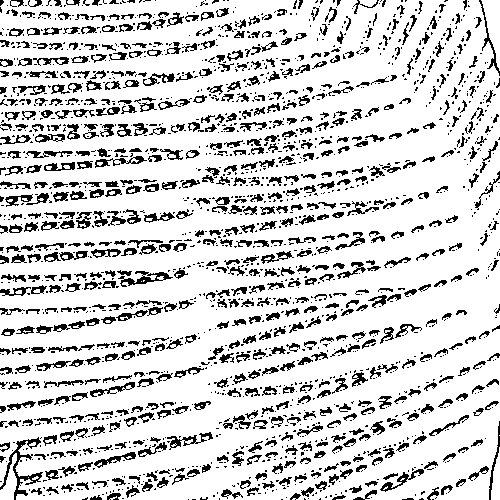
\includegraphics[width=.1\textwidth]{tbl/Tab_VerzElemente/V02a_PIK87-1-8-6.png} & Wiegeband mit Kamm \\
04.2 & 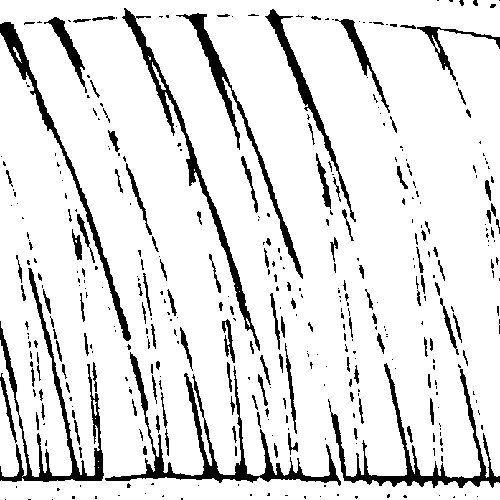
\includegraphics[width=.1\textwidth]{tbl/Tab_VerzElemente/V02b_MUN87-2-1-1-4-2.png} & Wiegeband (siehe Muster \enquote{IIIPla1z} von \textsc{Gouem Gouem} 2010/2011: 117 Abb. 9.3.a ) \\
04.3 & 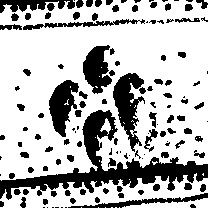
\includegraphics[width=.1\textwidth]{tbl/Tab_VerzElemente/V05e_INS87-102-2.png} & gruppierte Eindrücke \\
04.4 & 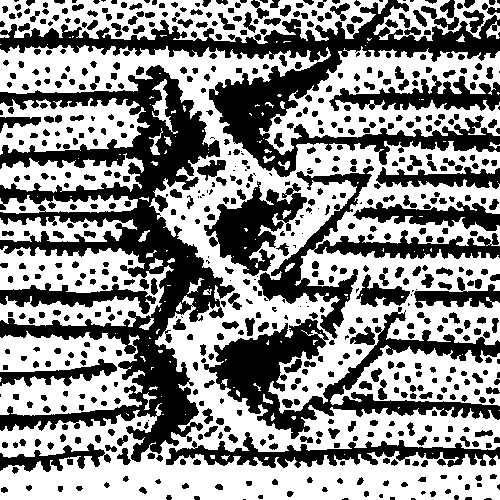
\includegraphics[width=.1\textwidth]{tbl/Tab_VerzElemente/V05f_SSL87-101-143.png} & gegenständige Eindrücke \\
04.5 & 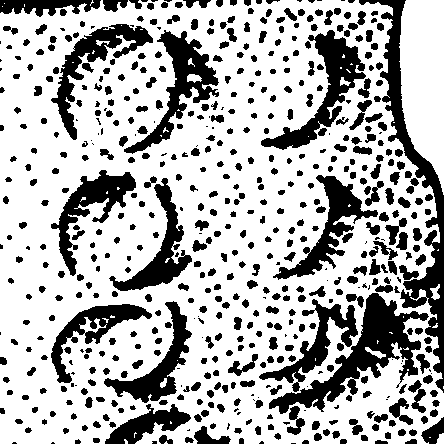
\includegraphics[width=.1\textwidth]{tbl/Tab_VerzElemente/V05j_SSL87-101-5.png} & kleine Flächen aus gegenständigen, halbrunden Eindrücken \\
04.6 & 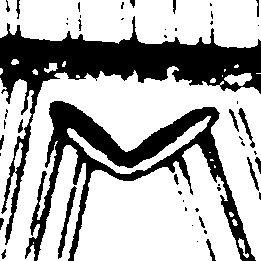
\includegraphics[width=.1\textwidth]{tbl/Tab_VerzElemente/V05h_DON85-102-a.png} & flache, winkelige Eindrücke \\
04.7 & 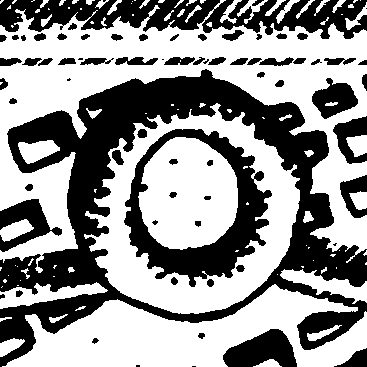
\includegraphics[width=.1\textwidth]{tbl/Tab_VerzElemente/V05i1_MLB85-1-2-3.png} & kleine Kreisaugen-Eindrücke \\
& & \\[1mm]
\bottomrule
\end{sftabular}}
\end{multicols}
\caption{Keramik: Verzierungselemente. Für die ersten beiden Stellen der Schlüsselzahl -- die  Verzierungstechnik -- siehe \textsc{Wotzka} (1995: 44 Tab.~3).}
\label{tab:Verzierungselemente}
\end{table*}

\addtocounter{table}{-1}
\begin{table*}[p]
\begin{multicols}{2}
\noindent
{\scriptsize\begin{sftabular}{@{}m{.05\columnwidth} m{.1\textwidth} m{.63\columnwidth}@{}}
\toprule
\multicolumn{2}{@{}l@{}}{\textbf{Schlüssel}} &  \textbf{Kurzbeschreibung} \\
\midrule
04.8 & 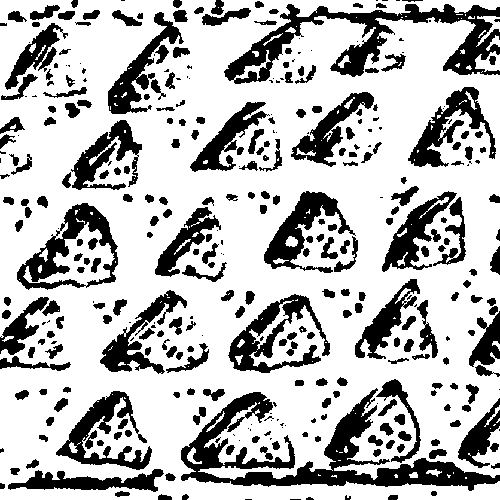
\includegraphics[width=.1\textwidth]{tbl/Tab_VerzElemente/V09l_MKA87-102-1.png} & dreieckige Eindrücke/Dreieckstempel \\
04.9 & 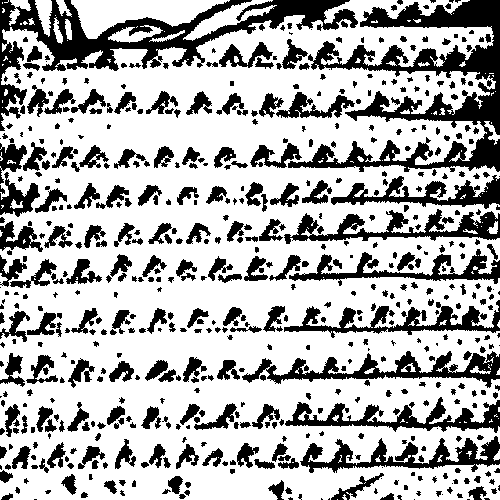
\includegraphics[width=.1\textwidth]{tbl/Tab_VerzElemente/V09j_MIS87-101-56.png} & flächig angeordnete, horizontale Bänder kleiner Eindrücke \\
04.10 & 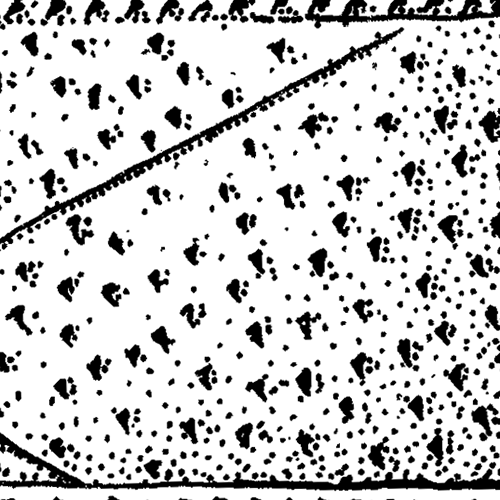
\includegraphics[width=.1\textwidth]{tbl/Tab_VerzElemente/V09k_MIS87-101-56.png} & lose flächig verteilte kleine Eindrücke \\
04.11 & 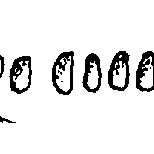
\includegraphics[width=.1\textwidth]{tbl/Tab_VerzElemente/V09i2_MKL85-101-114.png} & runde bis leicht ovale Eindrücke \\
04.12 & 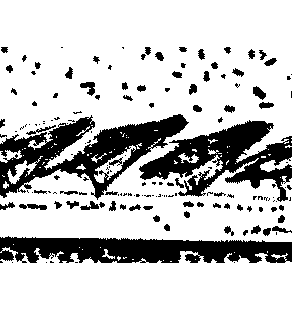
\includegraphics[width=.1\textwidth]{tbl/Tab_VerzElemente/V09a1_PIK87-1-14-1.png} & diagonale Eindrücke \\
04.13 & 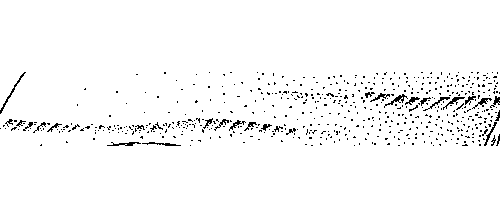
\includegraphics[width=.1\textwidth]{tbl/Tab_VerzElemente/V09n_SSL87-101-19.png} & leicht gewellte Bänder aus diagonalen oder vertikalen Eindrücken \\
04.14 & 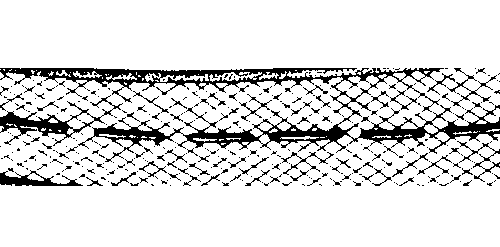
\includegraphics[width=.1\textwidth]{tbl/Tab_VerzElemente/V09a2_DON85-102-120.png} & horizontales oder vertikales Band aus linearen Eindrücken \\
04.15 & 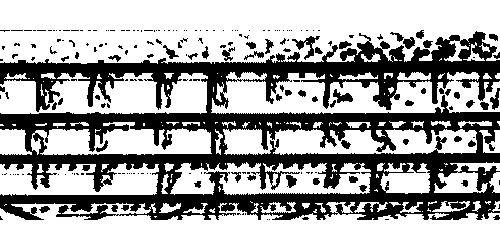
\includegraphics[width=.1\textwidth]{tbl/Tab_VerzElemente/V09b_PIK87-1-8-10.png} & vertikale Eindrücke \\
04.16 & 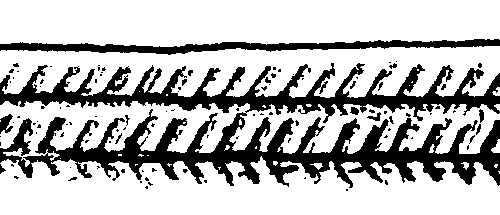
\includegraphics[width=.1\textwidth]{tbl/Tab_VerzElemente/V09c1_PIK87-1-13-1.png} 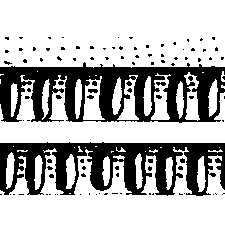
\includegraphics[width=.1\textwidth]{tbl/Tab_VerzElemente/V09c2_DON85-102-117.png} & Eindrücke in Rillen (siehe Muster \enquote{ISpeg5/ISpeg11} bei \textsc{Gouem Gouem} 2010/2011251, 251 Abb. 30.5) \\
04.17 & 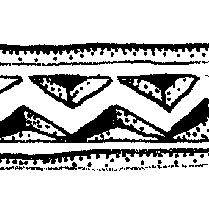
\includegraphics[width=.1\textwidth]{tbl/Tab_VerzElemente/V12b_INS87-102-2.png} & gegenständige Dreiecke in horizontalem Band \\
04.18 & 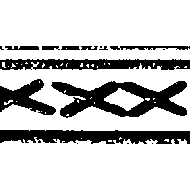
\includegraphics[width=.1\textwidth]{tbl/Tab_VerzElemente/V11b2_DON85-102-126.png} & Bänder aus x-förmigen Eindrücken \\
04.19 & 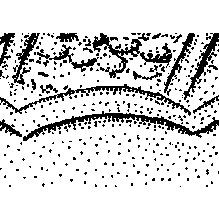
\includegraphics[width=.1\textwidth]{tbl/Tab_VerzElemente/V09h1_PDM87-101-12.png} & lange gebogene Eindrücke in Reihen \\
04.20 & 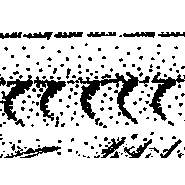
\includegraphics[width=.1\textwidth]{tbl/Tab_VerzElemente/V09h2_MIT87-102-19.png} & kurze gebogene Eindrücke (Fingernagel) \\
04.21 & 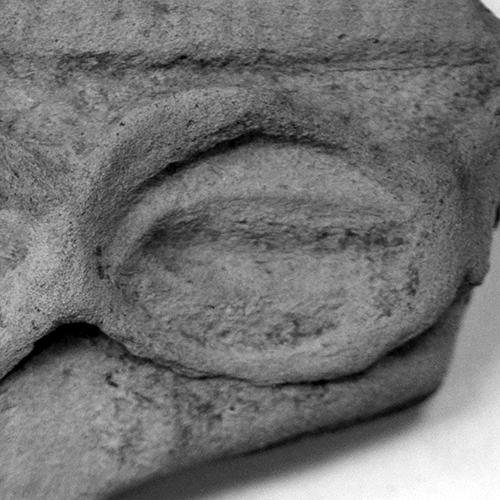
\includegraphics[width=.1\textwidth]{tbl/Tab_VerzElemente/V05i3_MBA11-1-1_DSC_0507_b.png} & Eindrücke mit Kaurischnecken oder Imitation \\
& & \\
\bottomrule
\end{sftabular}}

\noindent
{\scriptsize\begin{sftabular}{@{}m{.05\columnwidth} m{.1\textwidth} m{.63\columnwidth}@{}}
\toprule
\multicolumn{2}{@{}l@{}}{\textbf{Schlüssel}} &  \textbf{Kurzbeschreibung} \\
\midrule
05.1 & 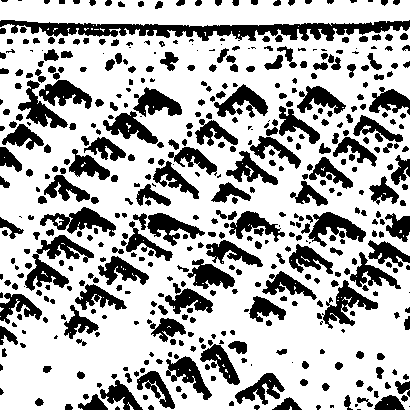
\includegraphics[width=.1\textwidth]{tbl/Tab_VerzElemente/V02c_PDM87-101-125.png} & diagonaler Kammeindruck \\
05.2 & 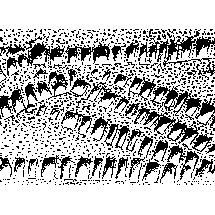
\includegraphics[width=.1\textwidth]{tbl/Tab_VerzElemente/V12a3_MKL85-101-105.png} & Band aus zickzackartig angeordneten Kammeindrücken \\
05.3 & 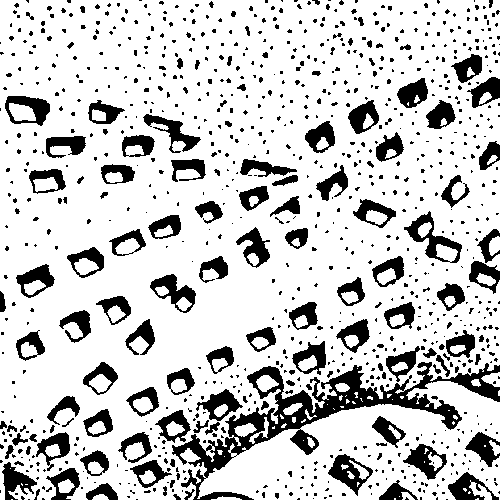
\includegraphics[width=.1\textwidth]{tbl/Tab_VerzElemente/V05a_PIK87-1-2-5.png} & Kammeindruck-Bänder \\
05.4 & 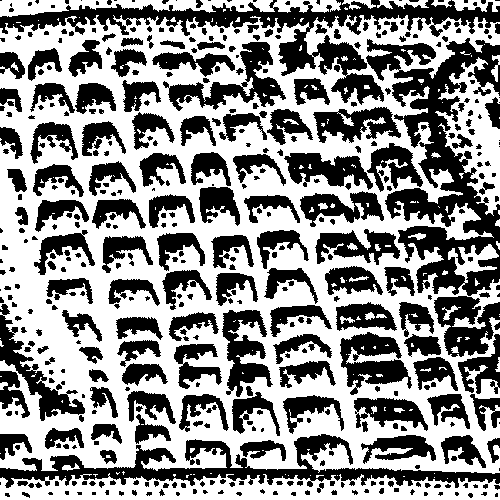
\includegraphics[width=.1\textwidth]{tbl/Tab_VerzElemente/V05b_PIK87-101-8.png} & flächiger Kammeindruck \\
08 & 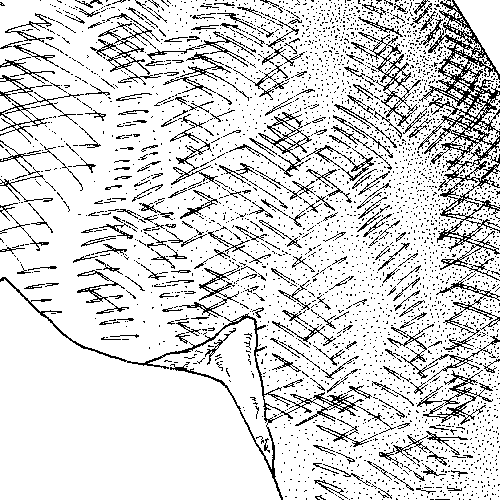
\includegraphics[width=.1\textwidth]{tbl/Tab_VerzElemente/V07_MUN87-1-0-2-3-6.png} & \textit{Bnfwa-nfwa} \parencite[Muster: siehe][109--111]{Wotzka.1995} \\
09.1 & 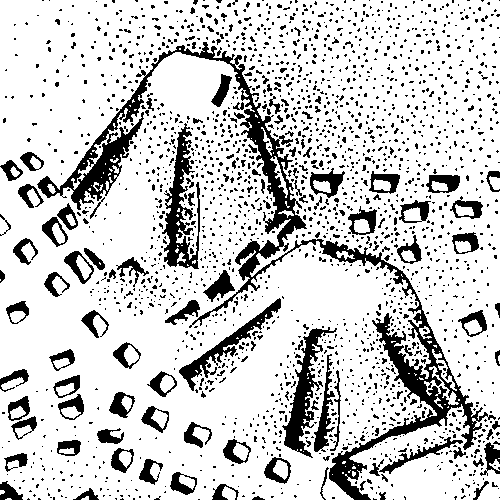
\includegraphics[width=.1\textwidth]{tbl/Tab_VerzElemente/V06a1_PIK87-1-2-5.png} & Knubben \\
09.2 & 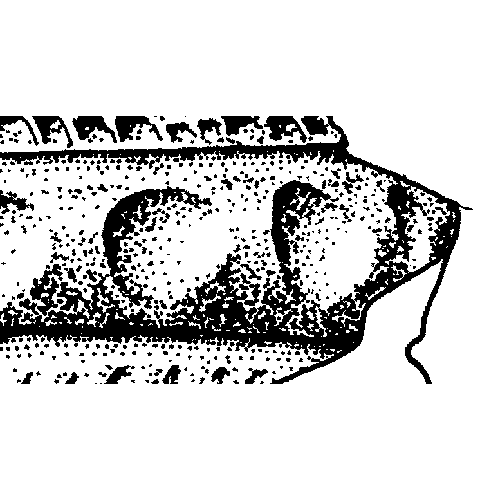
\includegraphics[width=.1\textwidth]{tbl/Tab_VerzElemente/V06b_PIK87-101-8.png} & Plastische Leiste \\
12 & 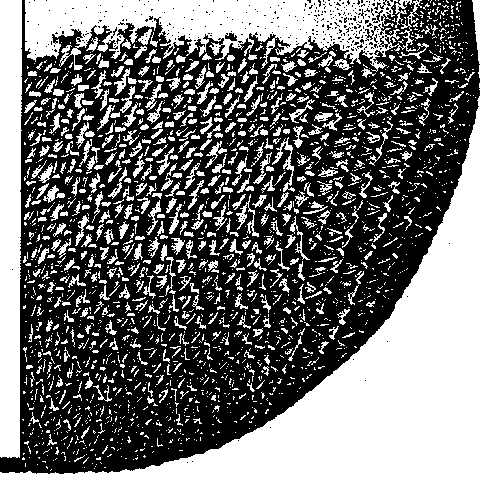
\includegraphics[width=.1\textwidth]{tbl/Tab_VerzElemente/V14_Wotzka1995_Taf91-4.png} & Mattenabdruck \\
13.1 & \includegraphics[width=.1\textwidth]{tbl/Tab_VerzElemente/V13_Gef3_CAM07-12-II-2.png} & Durchlochung der Gefäßwandung \\
14.1 & \includegraphics[width=.1\textwidth]{tbl/Tab_VerzElemente/VB1_YUM87-103-2.png} & Schwarze bis dunkelgraue Bemalung. Die Bemalung erfolgt ausschließlich in Streifen. Eine flächige Bemalung größerer Abschnitte eines Gefäßes wurde nicht beobachtet. \\
14.2 & \includegraphics[width=.1\textwidth]{tbl/Tab_VerzElemente/Vb2_BBS87-Herdgef_E87-04-4.png} & Rote Bemalung. Die Bemalung erfolgt ausschließlich in Streifen sowie in Riefen. Eine flächige Bemalung größerer Abschnitte eines Gefäßes wurde nicht beobachtet. \\
15.1 & \includegraphics[width=.1\textwidth]{tbl/Tab_VerzElemente/V04a_PIK87-1-3-5.png} & diagonaler Kammstrich \\
15.2 & \includegraphics[width=.1\textwidth]{tbl/Tab_VerzElemente/V04b_PIK87-1-2-225.png} & überkreuzter Kammstrich \\
& & \\[1.5mm]
\bottomrule
\end{sftabular}}
\end{multicols}
\caption{Keramik: Verzierungselemente. Für die ersten beiden Stellen der Schlüsselzahl -- die  Verzierungstechnik -- siehe \textsc{Wotzka} (1995: 44 Tab.~3).}
%\label{tab:Verzierungselemente}
\end{table*}

\addtocounter{table}{-1}
\begin{table*}[!tb]
\begin{multicols}{2}
\noindent
{\scriptsize\begin{sftabular}{@{}m{.05\columnwidth} m{.1\textwidth} m{.63\columnwidth}@{}}
\toprule
\multicolumn{2}{@{}l@{}}{\textbf{Schlüssel}} &  \textbf{Kurzbeschreibung} \\
\midrule
15.3 & \includegraphics[width=.1\textwidth]{tbl/Tab_VerzElemente/V05i2a_PIK87-101-17.png} \includegraphics[width=.1\textwidth]{tbl/Tab_VerzElemente/V05i2b_MTB85-101-12.png} & in Kammstrich-Technik hergestellte konzentrische, teilweise sich überlagernde Kreis-Muster \\
17.1 & \includegraphics[width=.1\textwidth]{tbl/Tab_VerzElemente/V06a2_MLB85-101-18.png} & Ösen \\
17.2 & \includegraphics[width=.1\textwidth]{tbl/Tab_VerzElemente/V06a3_LIB85-101-50.png} & Henkel \\
20.1 & \includegraphics[width=.1\textwidth]{tbl/Tab_VerzElemente/V08m_NGA87-101-22.png} & unklar, möglicherweise Mattenabdruck \\
20.2 & \includegraphics[width=.1\textwidth]{tbl/Tab_VerzElemente/V08n_MBK85-101-11.png} & unklar, möglicherweise Textilabdruck \\
21.1 & \includegraphics[width=.1\textwidth]{tbl/Tab_VerzElemente/V08a_BBL85-101-61.png} & \textit{knotted strip} \parencite[Muster: siehe][191 Abb.~1,C]{LivingstoneSmith.2007} \\
21.2 & \includegraphics[width=.1\textwidth]{tbl/Tab_VerzElemente/V08a1_LivingstoneSmith2007_Fig1A.png} & \textit{twisted string} (Muster: siehe \textsc{Livingstone Smith} 2007: 191 Abb.~1,A) \\
21.3 &  \includegraphics[width=.1\textwidth]{tbl/Tab_VerzElemente/V08a2_LivingstoneSmith2007_Fig1B.png} & \textit{alternate knotted strip} (Muster: ebd. 191 Abb.~1,B) \\
21.4 & \includegraphics[width=.1\textwidth]{tbl/Tab_VerzElemente/V08a3_Mayoretal2005.png} & \textit{Accordion-plaited strip} \parencite[Muster: siehe][36 Abb.~4]{Mayor.2005} \\
21.5 & \includegraphics[width=.1\textwidth]{tbl/Tab_VerzElemente/V08b_KPT85-101-10.png}  & Schnitzroulette, das ein Muster aus gegenläufigen gezähnten Bändern erzeugt \\
& & \\[5mm]
\bottomrule
\end{sftabular}}

\noindent
{\scriptsize\begin{sftabular}{@{}m{.05\columnwidth} m{.1\textwidth} m{.63\columnwidth}@{}}
\toprule
\multicolumn{2}{@{}l@{}}{\textbf{Schlüssel}} &  \textbf{Kurzbeschreibung} \\
\midrule
21.6 & \includegraphics[width=.1\textwidth]{tbl/Tab_VerzElemente/V08c_MTB85-101-94.png} & Schnitzroulette, das ein Muster aus gegenläufigen gezackten Bändern erzeugt \\
21.7 & \includegraphics[width=.1\textwidth]{tbl/Tab_VerzElemente/V08e_ILW85-101-11.png} & Schnitzroulette, das ein rautenförmiges Muster erzeugt, wobei das Zentrum erhaben ist \\
21.8 & \includegraphics[width=.1\textwidth]{tbl/Tab_VerzElemente/V08f_GBA85-101-6.png} & Schnitzroulette wie 21.7 jedoch mit einem erhabenen Zentrum und Grat \\
21.9 & \includegraphics[width=.1\textwidth]{tbl/Tab_VerzElemente/V08g_LIB85-101-28.png} & Schnitzroulette, das ein Muster aus dreieckigen Bändern erzeugt \\
21.10 & \includegraphics[width=.1\textwidth]{tbl/Tab_VerzElemente/V08h_BAT85-101-40.png} & Schnitzroulette wie 21.7 jedoch mit einem eingedrückten Zentrum \\
21.11 & \includegraphics[width=.1\textwidth]{tbl/Tab_VerzElemente/V08i_MBK85-101-15.png} & Schnitzroulette, das ein Muster aus konzentrischen Bögen erzeugt \parencite[Muster: siehe][191 Abb.~1,E]{LivingstoneSmith.2007} \\
21.12 & \includegraphics[width=.1\textwidth]{tbl/Tab_VerzElemente/V08j_NGA87-101-14.png}\hspace{1mm}\includegraphics[width=.1\textwidth]{tbl/Tab_VerzElemente/V08k_MBJ_E87-010-25.png} \includegraphics[width=.1\textwidth]{tbl/Tab_VerzElemente/V08l_MBJ_E87-010-27.png} & Schnitzroulette, das u.~a. ein tannenzweig-ähnliches Muster erzeugt \\
21.13 & \includegraphics[width=.1\textwidth]{tbl/Tab_VerzElemente/V09m_MTB85-101-37.png} & gebogene Eindrücke aus gegenständigen Dreiecken (rollrädchenartig) \\
22.1 & \includegraphics[width=.1\textwidth]{tbl/Tab_VerzElemente/VO1_PIK87-1-1-3.png} & Schlicker-Auftrag auf der Gefäßoberfläche \\
22.2 & \includegraphics[width=.1\textwidth]{tbl/Tab_VerzElemente/VO2_BAN85-501.png} & Aufrauung der Oberfläche. Das erzeugte Muster erinnert stark an \textit{Bnfwa-nfwa}-Verzierung (08), weist jedoch einen deutlich irreguläreren Verlauf der Eindrücke auf\\
\bottomrule
\end{sftabular}}
\end{multicols}
\caption{Keramik: Verzierungselemente. Für die ersten beiden Stellen der Schlüsselzahl -- die  Verzierungstechnik -- siehe \textsc{Wotzka} (1995: 44 Tab.~3).}
%\label{tab:Verzierungselemente}
\end{table*}



%\begin{sidewaysfigure*}[p]